\bookchapter{Kapitel 37: Paradigmenrevolution – vom „Code schreiben“ zum „KI anleiten“}

\chapterintro{Glückwunsch: Wer dieses Buch aufschlägt, steht mitten in einer beruflichen Paradigmenrevolution. Ihr Anfangspunkt: ein Satz eines Entwicklers in sozialen Medien im Jahr 2025. Klingt dramatisch? Ist aber so.}

\booksection{Die Geburt von Vibe Coding: Ein Satz startet eine Bewegung}

Im Februar 2025 schrieb Andrej Karpathy – merken Sie sich den Namen, er taucht noch öfter auf – in sozialen Medien einen oft zitierten Beitrag: „Es gibt eine neue Art zu programmieren: Vibe Coding. Man geht ganz nach Gefühl (vibes), ignoriert Code-Details und lässt die KI alles machen. Was man sieht, sagt man, kopiert, fügt ein – Hauptsache, es läuft.“

Dieser beiläufige Satz benannte präzise einen bereits laufenden Paradigmenwechsel: Menschen schreiben nicht mehr Zeile für Zeile Code, sondern beschreiben Absichten in natürlicher Sprache – die KI setzt um. Karpathys Formulierung war augenzwinkernd, dahinter steckt eine tiefere Einsicht: Sobald die Codegenerierung eine gewisse Schwelle überschreitet, ist der Engpass nicht mehr „Kann ich diese Zeile schreiben?“, sondern „Habe ich die Sache wirklich durchdacht?“.

\begin{tcbinfo}{Kurz erklärt: Was heißt Vibe?}
Vibe heißt wörtlich „Atmosphäre, Gefühl“. Vibe Coding ist also „nach Gefühl KI programmieren lassen“ – Sie beschreiben, was Sie wollen, die KI setzt es um. Merken Sie sich den Begriff, er ist die „Geburtsurkunde“ dieser Revolution.

\end{tcbinfo}

Seitdem spaltet sich die Bedeutung von „Kodieren“: Klassisch ist es Übersetzen von Design in Syntax; neu ist es Übersetzen von Absicht in Anweisungen. Ersteres fordert die Finger, letzteres den Kopf.

Vibe Coding wurde schnell vom Scherz zum seriösen Ingenieurkonzept. Mitte 2026 ist daraus eine vollständige Methodik geworden – von der Anforderungsformulierung über Kontextmanagement und iterative Verifikation bis zur Qualitätssicherung. Auch wurde klar: „Nach Gefühl“ ist nur der Einstiegszustand; hocheffektive KI-Programmierung braucht systematisches Denken. Genau das vermittelt dieses Buch.

\booksection{Stand 2026: Das Zeitalter von Agentic Engineering}

Bis August 2026 hat die KI-Programmierung mehrere Paradigmen durchlaufen. Vibe Coding war der erste Funke, doch bald zeigte sich: Nur „nach Gefühl“ mit der KI zu chatten liefert sehr ungleiche Qualität – mal brillant, manchmal katastrophal. Das Paradigma entwickelte sich weiter: von einfacher dialogbasierter Programmierung zu strukturierter Agent-Engineering.

Wieder Karpathy: Anfang 2026 prägte er den Begriff Agentic Engineering. Anders als Vibe Coding („sagen und generieren“) betont Agentic Engineering: Der KI ein Ziel geben, damit sie Schritte selbst plant, Werkzeuge aufruft, Ergebnisse prüft und nachbessert. Die KI ist kein reiner Codegenerator mehr, sondern ein Agent, der Umgebung wahrnimmt, Entscheidungen trifft und handelt.

Drei entscheidende Veränderungen:

\begin{enumerate}
  \item Interaktion: Von „Frage-Antwort“ zu „Ziel setzen und freigeben“.
  \item Arbeitsergebnis: Von „einem Codeabschnitt“ zu „einem vollständigen Projekt“.
  \item Rolle des Menschen: Von „Code Zeile für Zeile prüfen“ zu „Grenzen definieren, Ergebnisse abnehmen“.
\end{enumerate}

Zahlen lügen nicht: In Cursor 3 (April 2026) überholte der Agent-Modus erstmals die Tab-Vervollständigung – ein Zeichen für den massiven Umbruch in der Entwicklerarbeit. Claude Code, das terminalnahe KI-Programmierwerkzeug, erreichte Mitte 2026 einen Jahresumsatz von 2,5 Milliarden US-Dollar. Das folgende Schaubild zeigt den Wendepunkt:

\begin{center}
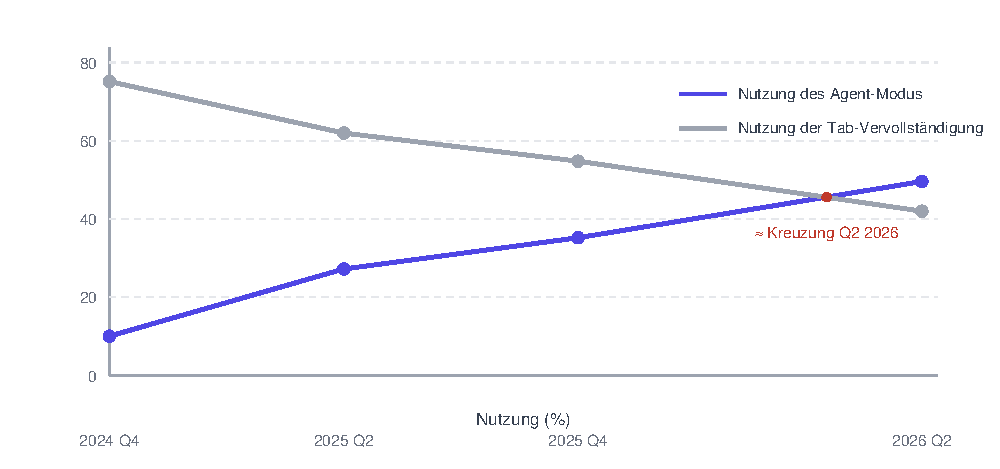
\includegraphics[width=0.92\linewidth]{figures/fig-di-san-shi-qi-zhang-1}
\\[2pt]\small Abbildung 1: Nutzung der Interaktionsmodi in der KI-Programmierung (Schätzung aus Branchendaten; Q2 2026 überholt Agent-Modus die Tab-Vervollständigung)
\end{center}

Ehrlich gesagt: Werkzeuge und Modelle sind nur Oberfläche. Ob Cursor oder Claude Code, ob GPT-5 oder Claude 4.5 – erfolgreiche Praktiker folgen derselben Grundmethodik. Genau die lehrt dieser Leitfaden.

\booksection{Der Kernwandel: Vom Coder zum Conductor}

Klassische Programmierlehre macht Sie zum Coder – Syntax verstehen, APIs lernen, Logikfehler debuggen. Im Zeitalter der KI-Programmierung wird die Rolle neu definiert: Sie müssen nicht mehr jede Zeile schreiben, aber zum „Dirigenten“ (Conductor) werden: Schlachtfeld definieren, Regeln setzen, Aufgaben verteilen, Ergebnisse abnehmen.

Der Kern liegt nicht darin, ob Sie Code schreiben können, sondern ob Sie klar denken können, was zu tun ist. Ein guter Dirigent ist nicht unbedingt der beste Soldat, kennt aber Ziel, Gelände und Truppenstärke am besten. So muss ein guter KI-Programmierer nicht jede Syntaxdetails beherrschen, aber Ziele, Architektur und Qualitätsmaßstäbe des Projekts genau kennen.

Diese Tabelle lohnt einen zweiten Blick – sie fasst den Rollenwandel zusammen:

\begin{center}
\begin{tabularx}{\linewidth}{|X|X|X|}
\hline
\textbf{Dimension} & \textbf{Klassischer Coder} & \textbf{KI-Dirigent (Conductor)} \tabularnewline
\hline
Kernkompetenz & Syntax, API-Aufrufe, Debugging & Anforderungen definieren, Kontext steuern, Abnahme \tabularnewline
Arbeitsweise & Zeile für Zeile schreiben & Absicht beschreiben, Ergebnisse prüfen \tabularnewline
Qualitätssicherung & Selbst geschrieben, selbst im Blick & KI-Ergebnisse durch Tests und Reviews prüfen \tabularnewline
Wissen & Tiefe Beherrschung einer Sprache/eines Frameworks & Breites Technikverständnis, tiefes Verständnis der Fachlogik \tabularnewline
Engpass & Tippgeschwindigkeit und Syntaxgedächtnis & Klarheit des Denkens und Ausdrucksvermögen \tabularnewline
Fehlerquellen & Syntaxfehler, logische Lücken & Unklare Anforderungen, fehlender Kontext \tabularnewline
\hline
\end{tabularx}
\end{center}

\begin{center}\small\color{gray}Klassischer Coder vs. KI-Dirigent im Vergleich\end{center}

Damit ist nicht gesagt, dass Programmierwissen unwichtig wäre. Ganz im Gegenteil: Wer KI-Code lesen kann, kann ihn wirksam prüfen und korrigieren; wer Datenstrukturen und Algorithmen versteht, kann die Pläne der KI bewerten. Wissen bestimmt die „Leitungsgrenze“ – aber seine Rolle wechselt vom Ausführungswerkzeug zum Urteilskriterium.

\booksection{Warum Methodik wichtiger ist als Werkzeuge}

Tools iterieren alle drei Monate, Methoden entwickeln sich erst alle drei Jahre weiter. Die Bedienung eines Tools kann nach drei Monaten veraltet sein; ein Denkansatz hält drei Jahre später noch.

Viele fragen beim Einstieg zuerst: „Welches Werkzeug ist am besten?“, „Welches Modell ist am stärksten?“ Wichtige Fragen, aber falsch priorisiert. Die Tool-Landschaft von August 2026 ist eine andere als August 2025 – Trae, Qoder und andere kommen und gehen, Cursor wurde vom Plugin zur eigenständigen IDE und dann zu Cursor 3, Claude Code vom Experiment zum Terminal-Standard. Doch hinter der Umtriebigkeit blieben die Denkprinzipien der Erfolgreichen fast unverändert.

Deshalb verschwendet dieses Buch keinen Platz für Bedienungsanleitungen einzelner Tools – die veralten im Handumdrehen. Stattdessen liegt der Fokus auf einer erprobten Denkmethodik: Anforderungen denken, mit der KI kommunizieren, Ergebnisse prüfen, iterativ verbessern. Wer diese Methodik beherrscht, kommt mit jedem Werkzeug schnell zurecht; wer nur Bedienung lernt, beginnt beim Toolwechsel bei null.

\begin{tcbinfo}{Beruhigung für Anfänger}
Wenn Sie neu einsteigen, lassen Sie sich vom Wort „Methodik“ nicht einschüchtern. Methodik ist keine abstrakte Philosophie, sondern ein Handbuch fürs Denken bei Problemen. Wie beim Kochen: Sie können einem Rezept folgen (Werkzeugbedienung), aber ein guter Koch versteht, „warum so würzen“ und „wie die Hitze steuern“ (Methodik). Dieses Buch erklärt die Grundlagen, jedes Prinzip mit konkreten Gegenbeispielen – damit Sie nicht nur verstehen, was gemeint ist, sondern wissen, wie es geht.

\end{tcbinfo}

\begin{tcbpractice}{Übung: Ihr persönliches „Rollenfoto“}
Nehmen Sie ein Blatt und beantworten Sie drei Fragen: (1) Wie nutzen Sie bisher KI beim Programmieren (falls überhaupt)? (2) Ähneln Sie eher dem „Coder“ oder dem „Dirigenten“ aus der Tabelle? (3) Wie würden Sie Ihre Arbeitsweise in drei Monaten beschreiben? Legen Sie den Zettel ins Buch und schauen Sie nach Kapitel 47 noch einmal herein – die Veränderung geht schneller, als Sie denken.

\end{tcbpractice}

\begin{tcbsummary}{Kapitel-Zusammenfassung}
\begin{itemize}
  \item 2025 nannte Karpathy die KI-Programmier-Revolution „Vibe Coding“: nicht Zeile für Zeile, sondern Absichten in natürlicher Sprache
  \item 2026 Weiterentwicklung zu Agentic Engineering: Ziel setzen, freigeben, KI plant und handelt, Mensch nimmt ab
  \item In Cursor 3 überholt der Agent-Modus erstmals die Tab-Vervollständigung; Claude Code bei 2,5 Mrd. USD Jahresumsatz
  \item Ihre neue Rolle: Conductor – Schlachtfeld definieren, Regeln setzen, Aufgaben verteilen, Ergebnisse abnehmen
  \item Werkzeuge entwickeln sich alle drei Monate, Methodik nur alle drei Jahre – Methodik lernen statt Bedienung
\end{itemize}

\end{tcbsummary}
